%!TEX root = paper.tex
\section{Evaluation}
\label{sec:eval}

\begin{figure*}
\centering
    \subfigure[LDA]{
        \label{fig:exp_lda}
        %\includegraphics[width=0.3\linewidth]{figures/fig_10B17_case1}
        \includegraphics[width=0.3\linewidth]{figs/exp_lda.eps}
    }
    \subfigure[SLDA]{
        \label{fig:exp_slda}
        %\includegraphics[width=0.3\linewidth]{figures/fig_15B31_case2}
        \includegraphics[width=0.3\linewidth]{figs/exp_slda.eps}
    }
    \subfigure[DCMLDA]{
        \label{fig:exp_dcmlda}
        %\includegraphics[width=0.3\linewidth]{figures/fig_48B48_case6}
        \includegraphics[width=0.3\linewidth]{figs/exp_dcmlda.eps}
    }
	\caption{Running Time}
    \label{fig:exp_comparison}
\end{figure*} 

In this section, we first present performance evaluation of InferSpark, 
based on constructing and carrying out statistic inference on five models that
are supported by the current InferSpark implementation: 
Latent Dirichlet Allocation (LDA), Gaussian Mixture Model, Bayes Point
Machine, Sentence-LDA (SLDA) \cite{Jo2011}, and Dirichlet Compound Multinomial
LDA (DCMLDA) \cite{Doyle2009}.
LDA is a standard model in topic modeling, which takes in a collection of documents
and infers the topics of the documents.  
\ZY{Brief Introduction to GMM and BPM}
The other two models are cutomized models that tweaks LDA according to the
characteristics of specific situations.
Sentence-LDA (SLDA) is a model for finding aspects in online reviews, which takes in online reviews, and infers the aspects.
Dirichlet Compound Multinomial LDA (DCMLDA) is another topic model that accounts for burstiness in documents.
All models can be implemented in InferSpark using less than 9 lines of code. 
%(see \figref{fig:intro_lda_def} and Appendix \ref{models}).
For comparison, we include MLlib in our study whenever applicable.
MLlib includes LDA as standard models.  However, MLlib does not include SLDA and DCMLDA.
There are other probabilistic programming frameworks apart from Infer.NET (see Section \ref{sec:related}).
All of them are unable to scale-out onto multiple machines yet.  
Infer.NET so far is the most predominant one with the best performance, so we also include it in our study whenever applicable.

All the experiments are done on nodes running Linux with 2.6GHz quad-core, 32GB memory, and 700GB hard disk. 
Spark 1.4.1 with scala 2.11.6 is installed on all nodes.
The default cluster size for InferSpark and MLlib is 24 data nodes and 1 master node.
Infer.NET can only use one such node.
The data for running LDA, SLDA, and DCMLDA are listed in Table \ref{data}.
The wikipedia dataset is the wikidump. Amazon is a dataset of Amazon reviews
used in \cite{Jo2011}.
We run 50 iterations and do checkpointing every 10 iterations for each model on each dataset.

Then we show how the partitioning strategy and GraphX optimization improve the
scalability of InferSpark. In these experiments, no checkpoints are taken.

\ZY{TODO: re-do scale-out experiment}

\ZY{TODO: do GMM and BPM experiment}

\begin{table}\scriptsize
\caption{Datasets}
\label{data}
\small
\begin{tabular}{ccc}
     \begin{tabular}{|c|c|c|}     \hline
        {Wikipedia} & words & topics \\\hline\hline
         0.2\% & 541,644 & 96 \\\hline
         0.5\% & 1,324,816  & 96 \\         \hline
         \multicolumn{3}{c}{LDA} \\
     \end{tabular}
          &
     \begin{tabular}{|c|c|c|}     \hline
        {Amazon} & words & topics \\\hline\hline
         6\% & 349,569 & 96 \\\hline
         10\% & 607,430  & 96 \\         \hline
         \multicolumn{3}{c}{SLDA} \\
     \end{tabular}
     \\\\
     \multicolumn{2}{c}{
     \begin{tabular}{|c|c|c|}     \hline
        {Wikipedia} & words & topics \\\hline\hline
         0.5\% & 1,324,816 & 10 \\\hline
         1\% & 2,596,155  & 10 \\         \hline
         \multicolumn{3}{c}{DCMLDA} \\
     \end{tabular}
     }
\end{tabular}
\end{table}

\subsection{Overall Performance}


\figref{fig:exp_comparison} shows the time of running LDA, SLDA, and DCMLDA 
on InferSpark, Infer.NET, and MLlib.
Infer.NET cannot finish the inference tasks on all three models within a week.
MLlib supports only LDA, and is more efficient than InferSpark in that case.
However, we remark that MLlib uses the EM algorithm which only
calculates Maximum A Posterior instead of the full posterior and is specific to LDA.
In contrast, InferSpark aims to provide a handy programming platform for statistician and domain users to build and test various customized models based on big data.
It would not be possible to be done by any current probabilistic frameworks nor with Spark/GraphX directly unless huge programming effort is devoted.  
MLlib versus InferSpark 
is similar to C++ programs versus DBMS: highly optimized C++ programs are more efficient, 
but DBMS achieves good performance with lower development time.
From now on, we focus on evaluating the performance of InferSpark.



Table \ref{breakdown} shows the time breakdown of InferSpark.
The inference process executed by GraphX, as expected, dominates the running time.
The MPG construction step executed by Spark, can finish within two minutes.
The Bayesian network construction and code generation can be done in seconds.


\begin{table*}
\caption{Time Breakdown (in seconds and \%)}
\label{breakdown}
\small
\begin{tabular}{|l||*{8}{r|}r|}
\hline
Model & \multicolumn{2}{c|}{B.N. Construction} & \multicolumn{2}{c|}{Code Generation}	& \multicolumn{4}{c|}{Execution} & Total \\\cline{6-9} 
  & \multicolumn{2}{c|}{ } & \multicolumn{2}{c|}{ }	& \multicolumn{2}{c|}{MPG Construction} & \multicolumn{2}{c|}{Inference} &	 \\ \hline \hline
LDA 541644 words	& 21.911	& 1.34\%	& 11.15 &	0.68\%	& 38.147	& 2.33\% &	1566.692 & 95.65\%	& 1637.9 \\ \hline
LDA 1324816 words &	21.911 & 0.70\% & 12.25	& 0.39\% & 79.4 & 2.55\%	& 3002.1 & 96.36\% &	3115.661 \\ \hline
SLDA 349569 words &	21.867 & 1.76\% & 11.05 &	0.89\%	& 26.33 & 2.12\% &	1182.2	& 95.23\%	& 1241.447 \\ \hline
SLDA 607430 words & 21.867 & 0.96\%	& 11.69	& 0.52\% & 41.152	& 1.81\%	& 2193.391	& 96.71\%	& 2268.1 \\ \hline
DCMLDA 1324816 words & 22.658 & 0.65\%	& 10.52 & 0.30\% &	20.923	& 0.60\% & 3448.699	& 98.46\% &	3502.8 \\ \hline
DCMLDA 2596155 words & 22.658 & 0.28\% & 11.55 & 0.14\%	& 39.549 & 0.48\%	& 8153.969 & 99.10\%	& 8227.726 \\ \hline

\end{tabular}
\end{table*} 





\subsection{Scaling-Up}

\figref{fig:scale-up} shows the total running time of LDA, SLDA, and DCMLDA on InferSpark
by scaling the data size (in words).
InferSpark scales well with the data size.
DCMLDA exhibits even super-linear scale-up. This is because as the data size goes up, 
the probability of selecting larger documents goes up. Consequently,
the growth in the total number of random variables is less than proportional, which gives rise
to the super-linearity.

\begin{figure}[h]\centering
	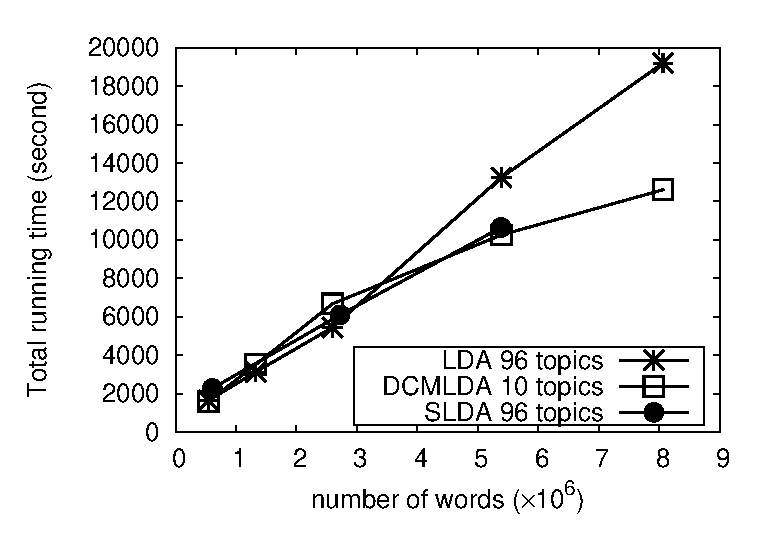
\includegraphics[width=0.35\textwidth]{figs/exp_lda_datasize.eps}
	\caption{Scaling-up}
	\label{fig:scale-up}
\end{figure}



\subsection{Scaling-Out}

\figref{fig:scale-out} shows the total running time of LDA on InferSpark in
different cluster sizes. For each model, we use fixed size of dataset.  DCMLDA
and LDA both use the 2\% Wikipedia dataset. SLDA uses the 50\% amazon dataset.
We observe that InferSpark can achieve linear scale-out. 

\begin{figure}[h]
	\centering
	\includegraphics[width=0.35\textwidth]{figs/exp_clustersize.eps}
	\caption{Scaling-out}
	\label{fig:scale-out}
\end{figure}


\subsection{Partitioning Strategy}

\figref{fig:exp_partition_strategy} shows the running time of LDA(0.2\% Wikipedia dataset, 96 topics) on InferSpark
using our partitioning strategy  and 
GraphX partitioning strategies: 
EdgePartition2D  (2D)
RandomVertexCut (RVC),
CanonicalRandomVertexCut (CRVC), and
EdgePartition1D (1D).
We observe that the running time is propotional to the size of EdgeRDD.
Our partition strategy yields the best performance for running VMP on the
message passing graphs.  Our analysis shows that RVC and CRVC should have the
same results. The slight difference in the figure is caused by the randomness
of different hash functions.


\begin{figure}[h]\centering
	\includegraphics[width=0.35\textwidth]{figs/exp_partition_strategy.eps}
	\caption{Different Partition Strategies}
	\label{fig:exp_partition_strategy}
\end{figure}

\subsection{Evaluation of the GraphX Optimizations}

We run the VMP implementation for LDA on different sizes of wikipedia dataset
using both GraphX and InferSpark-Graph for 10 iterations. The number of topics
is 96 and the vocabulary size is 9040. No checkpoint is made during the
execution. We measure the time of execution and the size of data shuffled in
each iteration.

\begin{figure*}[h]
\centering
	\subfigure[1st iteration time]{
		\label{fig:graph_cmp_first_iteration_datasize}
		\includegraphics[width=0.45\linewidth]{figs/graph_cmp_first_iteration_datasize.eps}
	}
	\subfigure[average iteration time excluding 1st iteration]{
		\label{fig:graph_cmp_average_iteration_datasize}
		\includegraphics[width=0.45\linewidth]{figs/graph_cmp_avg_iteration_datasize.eps}
	}
	\caption{Iteration time against data size of VMP for LDA using GraphX and
	InferSpark-Graph}
	\label{fig:graph_cmp_iteration_time_datasize}
\end{figure*}

\begin{figure*}[h]
\centering
	\subfigure[shuffle size]{
		\label{fig:graph_cmp_shuffle_size_datasize}
		\includegraphics[width=0.45\linewidth]{figs/graph_cmp_shuffle_size_datasize.eps}
	}
	\subfigure[total running time]{
		\label{fig:graph_cmp_total_time_datasize}
		\includegraphics[width=0.45\linewidth]{figs/graph_cmp_total_time_datasize.eps}
	}
	\caption{Total time and shuffle size against data size of VMP for LDA using GraphX and InferSpark-Graph}
\end{figure*}

\figref{fig:graph_cmp_iteration_time_datasize} shows the iteration time
comparison between GraphX and InferSpark-Graph by scaling up the data size.
Both the first iteration time and average iteration time 
using InferSpark-Graph is significantly shorter than that using
GraphX. When the data size increases, the iteration time increases linearly
using InferSpark-Graph while there is a super-linear increase of iteration
time using GraphX. It shows that InferSpark-Graph greatly improves the
scalability of InferSpark.

\figref{fig:graph_cmp_shuffle_size_datasize} shows the total size of data
shuffled among the workers in one iteration. The total size of data shuffled
using InferSpark-Graph is significantly smaller than that using GraphX. It
also reaches a fixed constant size as the data size increases in contrast of
the linear increase of the size of data shuffled using GraphX. This explains
why InferSpark-Graph could scale linearly but GraphX cannot: the shuffle in
InferSpark-Graph takes a fixed amount of time and the majority of time is
spent on computation while the shuffle in GraphX will eventually take the
majority of the time and thus incur too much system overhead.

Finally, \figref{fig:graph_cmp_total_time_datasize} shows the improvement of
total running time using InferSpark-Graph. Though the total running time
increases super-linearly using both frameworks, the InferSpark-Graph still
runs increasingly faster than GraphX as data size increases. The
super-linearity is caused by the graph construction phase, where the size of
data shuffled is huge and inevitable.

